To be able to track the interface between the blue core and the hot gaseous products a Level set method is used. The Level set method represents the interface by an implicit function $\phi$ defined as equation \ref{eq:levelsetmethod} in a 3D-space, where $h = 0$. 

\begin{subequations}
\label{eq:levelsetmethod}
\begin{equation}
 L = \left \{ \vec{x} \in \Re^3 : \phi(\vec{x}) = h  \right \}
\end{equation}    
\begin{equation}
  L_{inside} = \left \{ \vec{x} \in \Re^3 : \phi(\vec{x}) \geq h  \right \}
\end{equation}
\begin{equation}
  L_{outside} = \left \{ \vec{x} \in \Re^3 : \phi(\vec{x}) <  h  \right \}
\end{equation}
\end{subequations}

This representation is useful for tracking and calculating topology properties of a interface. The representation makes it easy to find out where in the fluid a sample point is taken since it is only a matter of testing the sign. Since $\phi$ is a implicit function, the normal can be calculated as in equation \ref{eq:normal1}.

\begin{equation}
\label{eq:normal1}
 \vec{n} = \frac{ \nabla \phi }{ \left | \nabla \phi \right | }
\end{equation}    

Moving an interface along a vector field $\vec{V}$, the velocity field for instance, is a matter of solving the hyperbolic PDE in equation \ref{eq:levelset_advection}.

 \begin{equation}
\label{eq:levelset_advection}
  \frac{\partial \phi}{\partial t} = -\vec{V} \cdot \nabla \phi
\end{equation}  

$\phi$ is also a signed distance function which means that the value of $\phi$ gives the distance to the closest point $\vec{p}$ of the interface, eq. \ref{eq:signed_distance}. The direction of this point is also parallel with the surface normal, and since the length of the gradient is $1$ \cite{bridson}, this point $\vec{p}$ can be calculated for a given point $\vec{x}$ by equation \ref{eq:find_point}.

\begin{subequations}
\label{eq:signed_distance}
\begin{equation}
distance_L(\vec{x}) = \underset{\vec{p} \in L}{min} \left \| \vec{x} - \vec{p} \right \|
\end{equation}    
\begin{equation}
\phi(\vec{x}) = distance_L(\vec{x}) : \vec{x} \text{ is inside}
\end{equation}
\begin{equation}
\phi(\vec{x}) = -distance_L(\vec{x}) : \vec{x} \text{ is outside}
\end{equation}
\end{subequations}

\begin{equation}
\label{eq:normal2}
 \vec{n} = \nabla \phi
\end{equation} 

\begin{equation}
\label{eq:find_point}
 \vec{p} = \vec{x} - \vec{n} \cdot \nabla\phi(\vec{x}), \vec{p} \in L
\end{equation}

\begin{figure}[h!]
	\centering
		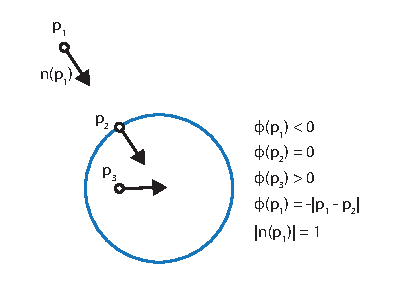
\includegraphics[width=.5 \linewidth]{figures/levelset.pdf}
	\caption{Illustration of the level set in 2D, and its properties.}
	\label{fig:levelset}
\end{figure}

\subsection{Reinitialize signed distance function}
Since the level set only is a sampled signed distance function in practice, a reinitialize operation is used to make sure that the level set is always close to a signed distance function. 
This is done by making sure that the length of the gradient is kept close to 1.
By always having the grid described in this way, it is certain that whenever moving in the direction of the gradient towards the surface with the distance $d$, the closest point on the surface will not change and the distance to the surface is now $d$ less then it was before.

Since the levelset is only a sampled signed distance function in practice, a reinitialize operation is used